\section{Requirements and Guidelines for iDACs}\label{sec:reqs}
Since creating, delivering, and supporting the implementation of LSST data products via iDACs creates some cost to the LSST Project, iDACs will be expected to follow some basic requirements and guidelines, which are described below.
The actual costs of iDAC support and infrastructure development are considered separately in Section \ref{sec:xfercost}.

\subsection{LSST site topology} \label{sec:topology}

Figure \ref{fig:idac-topology} shows a  topology for a set of interconnected iDACs.  US scientists will have direct access to the LSST Data Access Facility at NCSA.  Hosting on the cloud is shown, as described in 
	
\begin{figure}
\begin{center}
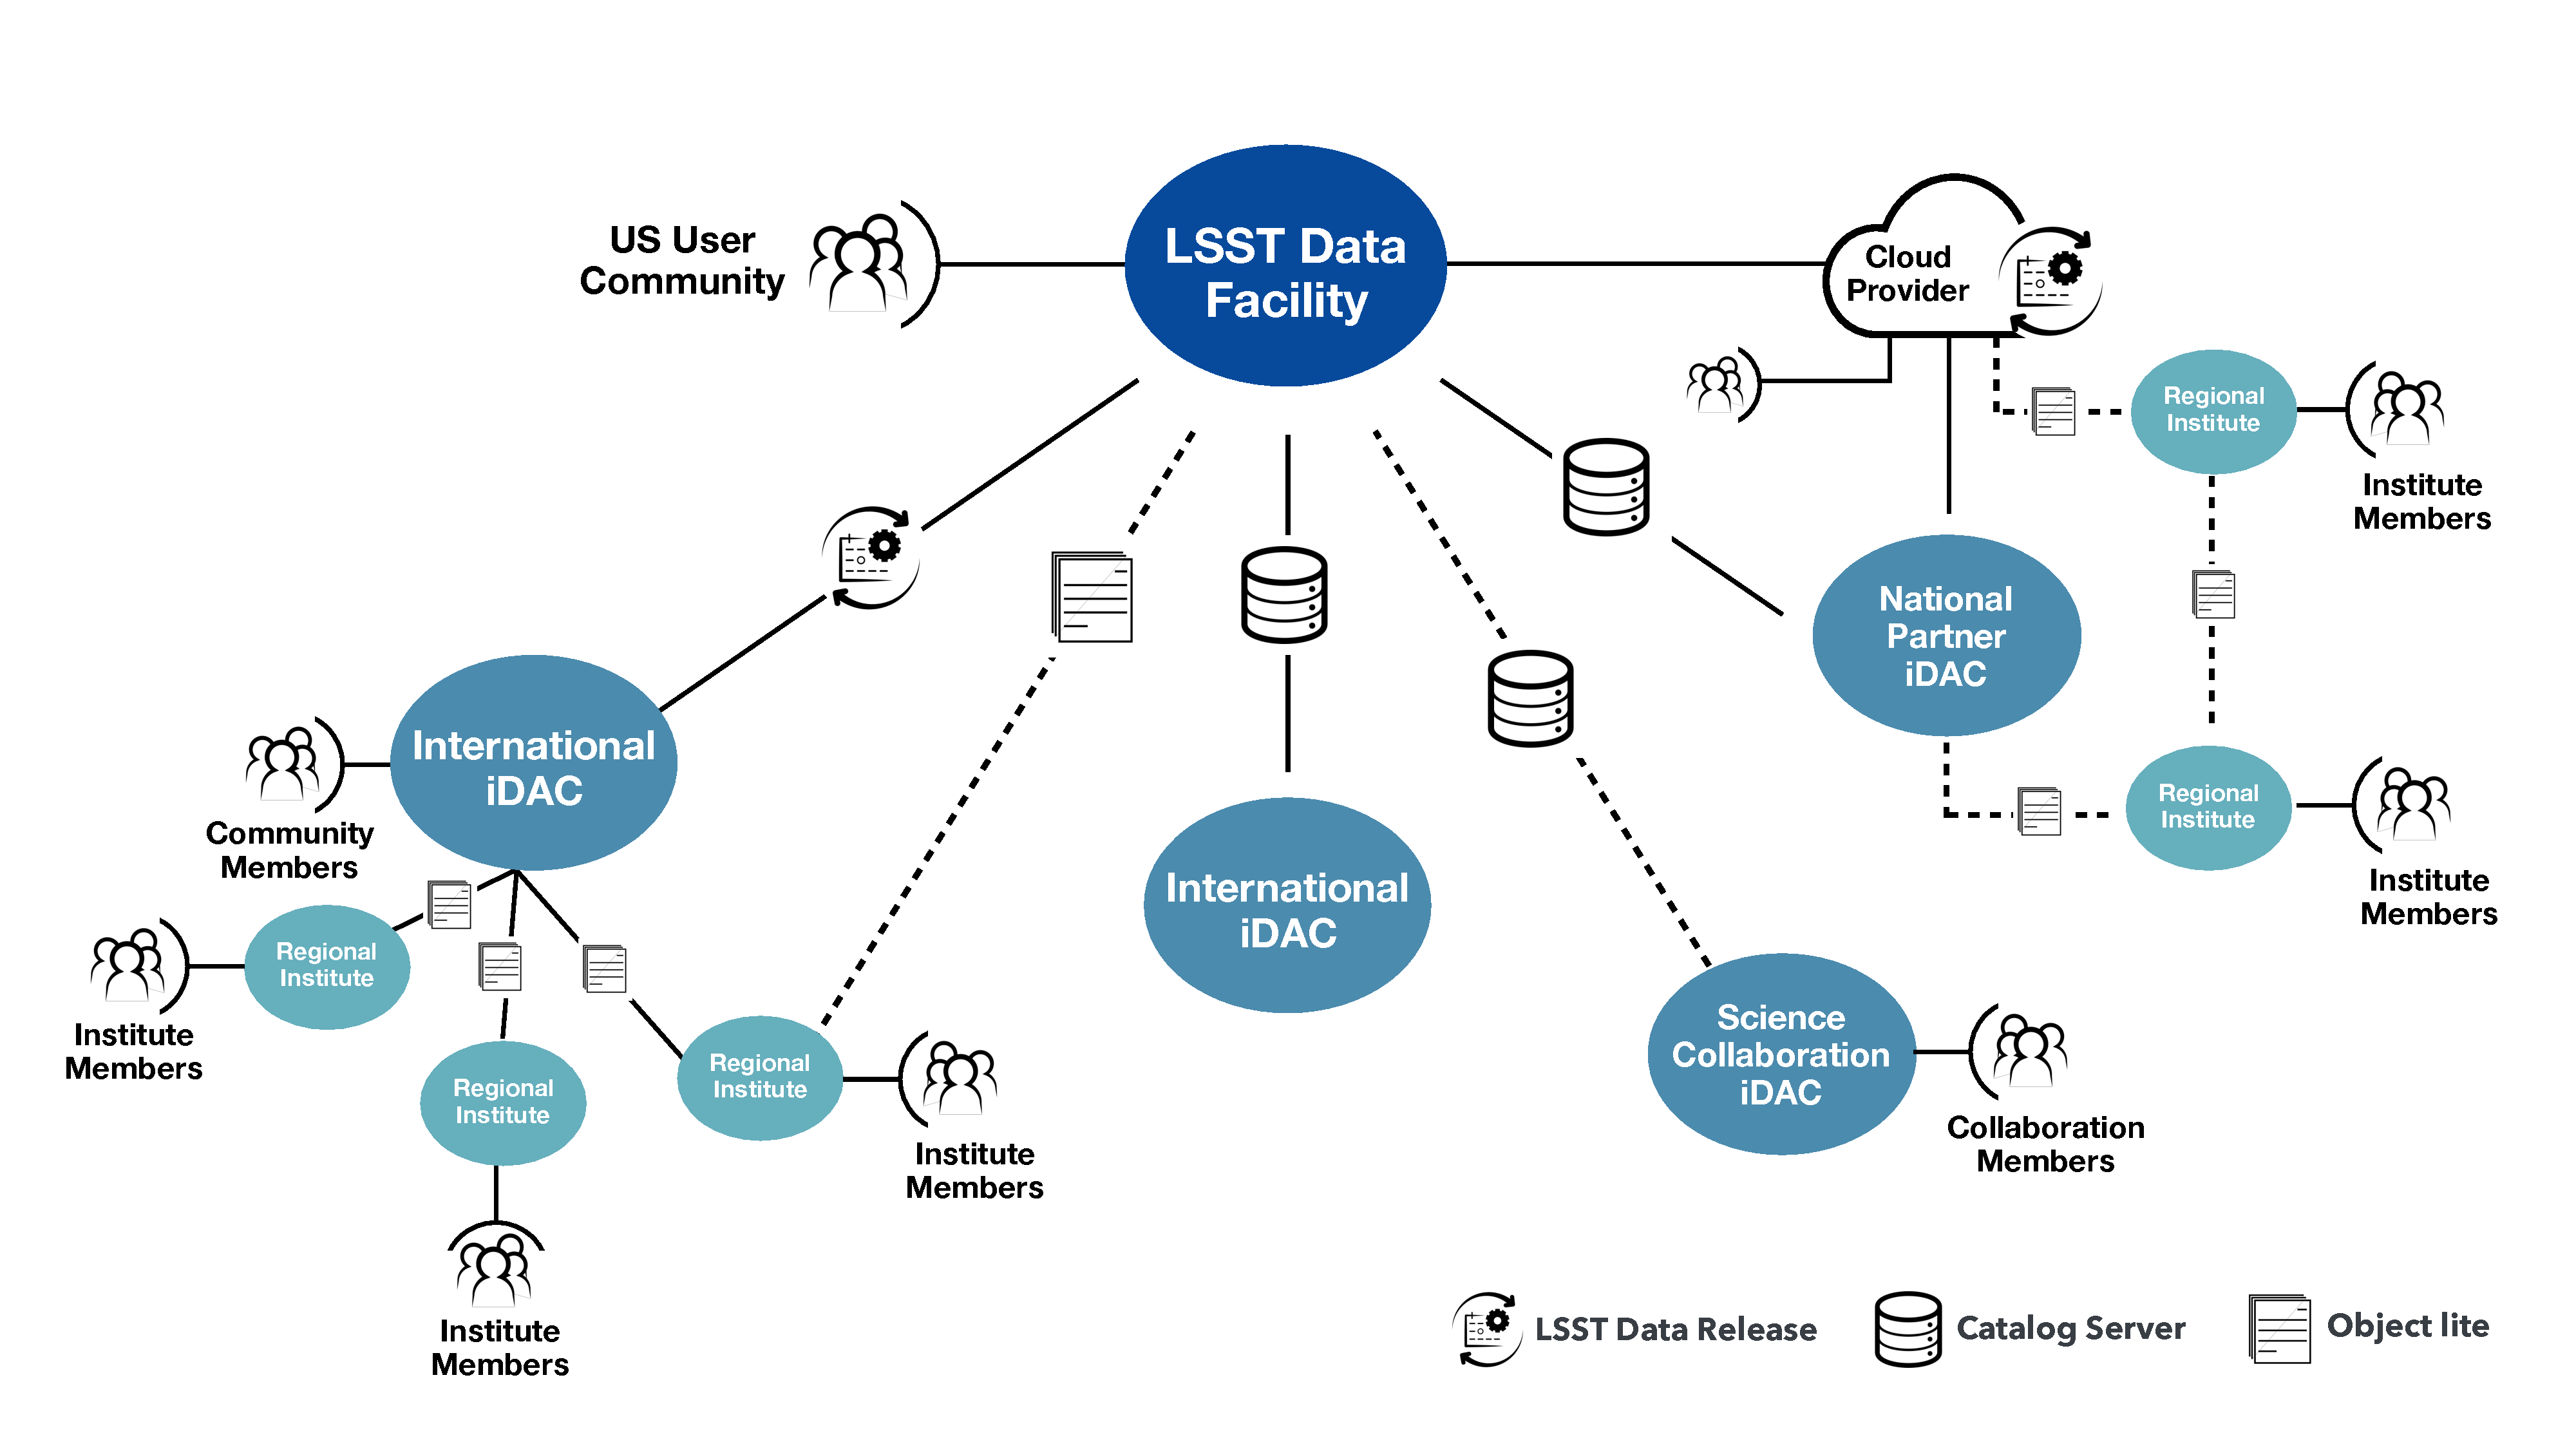
\includegraphics[width=0.95\textwidth]{images_local/idac-topology}
\caption{LSST Data Facility and Independent DAC network topology.  \label{fig:idac-topology}}
\end{center}
\end{figure}

\subsection{Required Resources} \label{sec:resources}
Institutions or organizations wishing to set up independent data access centres will be expected to have
sufficient resources and commitments before we discuss data transfers and support.
See also \secref{sec:cvs} for a discussion on compute vs storage.

\subsubsection{Data Storage}
Any institution considering setting up an iDAC will need to show commitment on purchasing sufficient storage and CPU power to hold and serve the data. Sufficient storage ranges from $0.5$ exabytes for the full data release(s) down to $100$ terabytes for a catalog server, and potentially further down to $70$ terabytes if the {\tt Object Lite} option is offered. For the full catalog , of order 100 nodes are required to serve it up. To serve images, a DAC would need some additional servers; depending on load this may be order 10 additional nodes.

\subsubsection{User Computational}
If the full set of data release products including images and catalogs are desired, it is highly recommended that the iDAC deploy the LSST Science Platform (LSP). The LSP serves as a portal to the data, and provides a user interface of web services and Jupyter notebooks for scientific queries and analysis, an open software framework for astronomy and parallel processing, and the associated computational, storage, and communications infrastructure needed to enable science. The LSP is described in full in \citeds{LSE-319} and \citeds{LDM-554}. Depending on the assumed load, the LSP is relatively modest as it requires only $\sim2$ servers to set up, and it is recommended to have 2 CPUs per simultaneous user (e.g., if the iDAC's desired capability is to serve 200 users, but only expect 50 to be active at a time, then 100 CPUs would be sufficient). From that starting point, the amount of next-to-the-data computational resources can be as large as the data center wishes to provide, and may make use of connecting to e.g., local super computer resources.

\subsubsection{Dedicated Personnel}
The significant hardware required by an iDAC is above the normal level for most astronomy departments, and would require dedicated technical personnel to set it up and keep it running. For an {\tt Object Lite} catalog running on existing hardware, this might not be a significant increase in person power if the hardware is already serving on order $50$--$100$ terabytes. Still, it is recommended to assume $\gtrsim0.25$ full-time equivalent (FTE) personnel hours for {\tt Object Lite}, and perhaps closer to $\sim2$ FTE for the full catalogs, which includes setting up and maintaining the service, and installing new data releases and software updates every year. For iDACs wishing to host the full data releases' images and catalogs and deploy the LSST Science Platform, it becomes necessary to employ $1$--$2$ storage engineers to mange the large amount of data, and possibly one more FTE to keep the Kubernetes (or equivalent) system updated with the latest software deploys. If the iDAC intends to support the science of many local users, support will become a specific issue which may not be covered by the usual institutional funding, and will require further effort. It is therefore recommended that any partner institution wishing to host a full-release iDAC provide a minimum personnel of 5 FTE to be considered viable.

\subsection{Networking and distribution}
There is an assumption than any prospective iDAC will have a high bandwidth connection with demonstrated sustained $40 Gb/s$ to enable data transfer and sufficient bandwidth for access by users.
In addition all iDACs should be ready  to serve the {\tt Object Lite} catalog to any institution worldwide but especially any {\em local} institutions.

\subsection{Services}

Independent DACs will be expected to provide services analogous to those provided at the LSST Data Facility at NCSA.  

\subsubsection{The LSST Science Platform}

The {\it LSST Science Platform}  \citeds{LSE-319} is a set of integrated web applications and services deployed at  LSST Data Access Centers through which the scientific community will access, visualize, subset and perform next-to-the-data analysis of the data collected by the LSST; it is envisioned to enable science cases that would greatly benefit from the co-location of user processing and LSST data. It will provide users access to the {\tt Data Products} described in \ref{sec:data}, such as, resources for image reprocessing, access to the LSST processing framework, and many other services as described in \citeds{LSE-163}.  All LSST {\tt Independent Data Access Centers} will be expected to run and support the LSST Science Platform. 

\subsubsection{User Generated data products }

{\it User Generated} data products will be created by the community deriving from the {\it Prompt} and {\it Data Release} data products, and making  full use of the power of the LSST database systems and
Science Platform for the storage, access, and analysis of their results.
The Science Platform will allow for the creation of {\it User Generated} data products and will enable science cases that greatly benefit from co-location of user processing and/or data within the LSST Archive Center.  Independent DACs will be expected to provide support for the creation of {\it User Generated} data products and their federation with the LSST Data products. 

\section{Responsibilities of the LSST Data Facility}

This section describes the services that the LSST Data Facility (LDF) will provide in support of all  iDACs.

The LDF will prepare data products for distribution to iDACs along with documentation of hardware and software that will make serving LSST data consistent with the serving of data from the LSST Data Facility. LSST will provide (modest) technical support consistent with available resources to assist groups setting up iDACs. 

LSST, through the LDF will establish a process for potential iDAC groups to interface with and establish data transfers to their iDACs. It is expected that iDAC groups will propose to LSST what their iDAC would support and then LSST will work with them to establish requirements to receive LSST data. One approved, LSST will provide (modest) technical support consistent with available resources to assist groups setting up their iDACs provided they comply with prerequisites discussed in this document and especially in \secref{sec:resources}.

\subsection{Proprietary Data Access Policies}
{\color{red}Defer for now until further guidance received.} \newline
=======

\subsection{Data Distribution} \label{sec:dist}

NCSA will have $100Gb/s$ connections  on ESNET which has interconnects with Internet2 - this should provide a distribution mechanism for getting data to iDACs, it will however be limited by the fact that much of our bandwidth is already allocated for data transmission to IN2P3 and alert distribution.

A tiered model as used by CERN for high energy physics would seem a desirable way to achieve big transfers. Hence we would have a small selection of tier 2 centres with all data products from which tier 3 centres could copy the subsets they wish to work with.  Other alternatives are discuss in \secref{sec:xfer}.

In HEP experiments such as  BABAR various physics analysis groups (science collaborations in LSST ) were assigned to specific international centers as their primary computing and analysis facility, thereby distributing the computing load around the "network." Users naturally tend to use the facility with available resources and cycles.
%National groups received credit against their normal "operating common fund" contributions (equivalent to part of the LSST operations cost) based on their local computing contribution, and service to the full collaboration (equivalent to the full LSST data rights community).
%We have not discussed  such system in place for LSST yet though.
~
%WOM - I took a go at it ..
%Points to be addressed
%\begin{enumerate}
%\item High-bandwidth network out of the LDF to all iDACs
%\item Distribution of each of the data products types outlined in \ref{sec:data} to iDACs
%\item ......
%\end{enumerate}


